% Main figure. Select the latest available carbon-constrained year per system.
\begin{figure}[p]
\centering
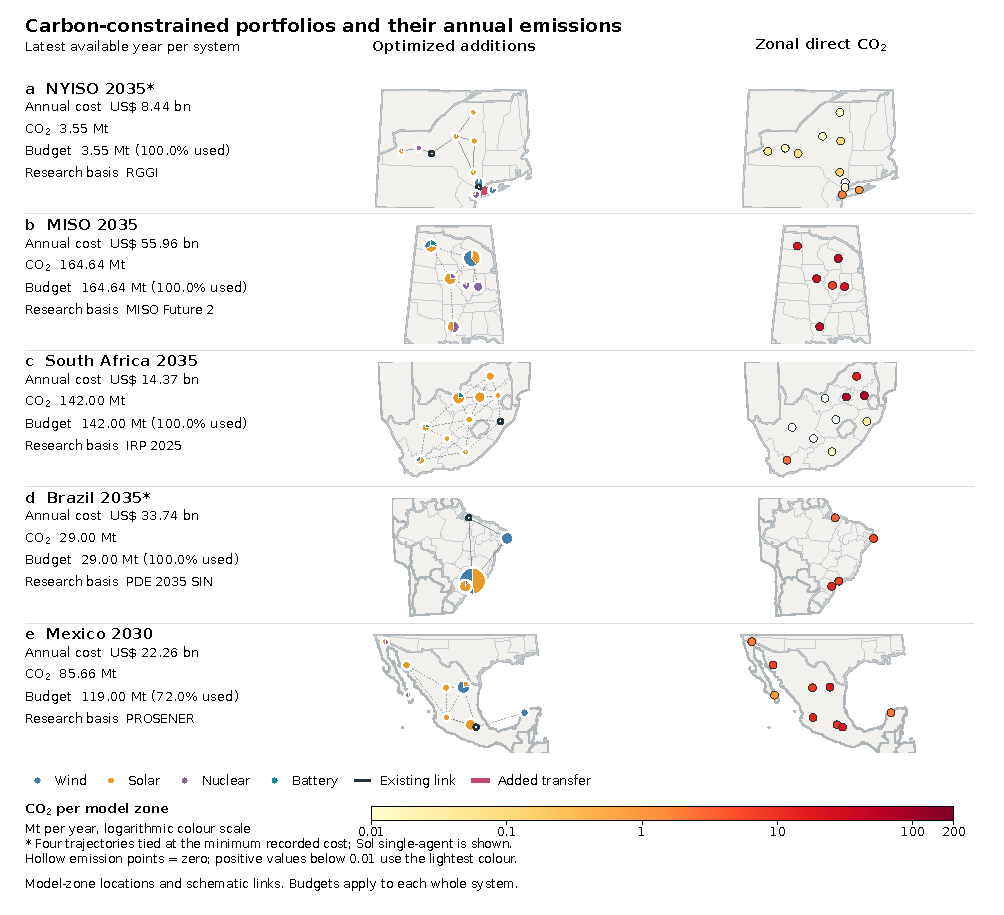
\includegraphics[width=170mm]{figure_carbon/combined_grid_carbon.pdf}
\caption{\textbf{Optimized grid additions and emissions under research carbon budgets.}
Panels show the lowest observed cost among four accepted trajectories for each system's latest available year, with GPT-6.1 Sol single-agent as the representative. NYISO and Brazil have tied minima. Left maps show added wind, solar, nuclear and battery power; pie area increases with total additions, retaining a minimum visible area. Grey links are existing model connections, dashed where ratings are assumed, and magenta links show added or official-project transfer. Right maps show direct annual generator CO$_2$ aggregated from the same candidate's 8,760-hour dispatch, using one logarithmic colour scale. Hollow emission points denote zero. Locations are model-zone representatives, not plant sites or a spatial emissions inventory. Cost, emissions, the system-wide budget and its research basis accompany each case. Budget definitions and source mappings are given in Methods.}
\label{fig:combined-grid-carbon}
\end{figure}

% Supplementary atlas has ten pages, in this order:
% 1 NYISO2023;2 NYISO2030;3 NYISO2035;4 MISO2030;5 MISO2035;
% 6 Mexico2030;7 Brazil2030;8 Brazil2035;9 SouthAfrica2030;10 SouthAfrica2035.
% Use \includegraphics[page=N,width=170mm]{figure_carbon/combined_grid_carbon_atlas.pdf}.
% Caption template:
% \caption{\textbf{Carbon-constrained grid additions and emissions for REGION YEAR.}
% The paired maps show the selected lowest-cost accepted candidate's added generation,
% storage and transfer capacity and its annual direct generator CO$_2$.
% Numbered model-zone locations link to the common numerical ledger.
% Existing denotes inherited generation, Energy denotes added battery energy,
% and emissions are summed from 8,760 one-hour dispatch snapshots.
% Both maps retain representative model-zone locations; connections are schematic.
% The research carbon budget applies to the entire system.
% Encodings and selection follow Fig.~\ref{fig:combined-grid-carbon}.}
